% Brecha ES vs EN — datos de doc/results/p2_baseline.json y p2_post.json
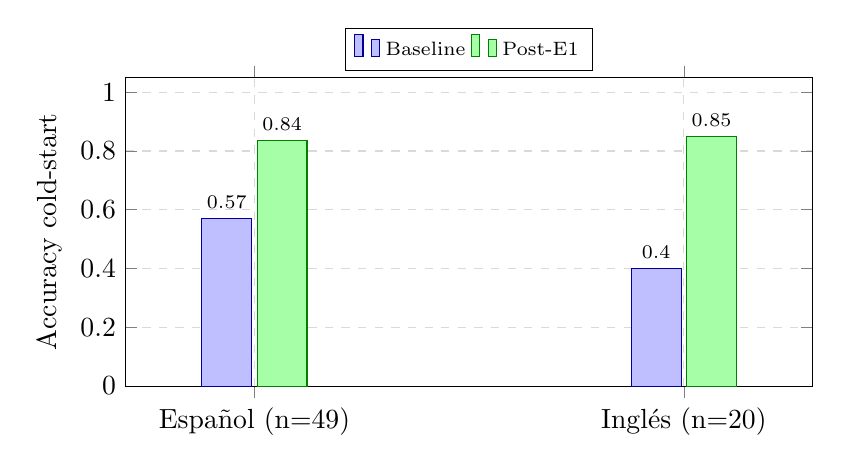
\begin{tikzpicture}
\begin{axis}[
    width=0.85\linewidth, height=5.5cm,
    ybar,
    bar width=18pt,
    ylabel={Accuracy cold-start},
    ymin=0, ymax=1.05,
    ytick={0,0.2,0.4,0.6,0.8,1.0},
    yticklabel={\pgfmathprintnumber[fixed,precision=2]{\tick}},
    symbolic x coords={Español (n=49), Inglés (n=20)},
    xtick=data,
    legend style={at={(0.5,1.02)},anchor=south,legend columns=2,font=\scriptsize},
    nodes near coords,
    nodes near coords style={font=\scriptsize},
    every node near coord/.append style={/pgf/number format/.cd, fixed, precision=2},
    grid=major,
    grid style={dashed, gray!30},
    enlarge x limits=0.3,
]
\addplot[fill=blue!25,draw=blue!60!black] coordinates {
  (Español (n=49),0.571) (Inglés (n=20),0.400)
};
\addplot[fill=green!35,draw=green!50!black] coordinates {
  (Español (n=49),0.837) (Inglés (n=20),0.850)
};
\legend{Baseline, Post-E1}
\end{axis}
\end{tikzpicture}
